\chapter{Background}

% In this chapter, all background necessary to understand the thesis are introduced. The level of detail is such that 
% a colleague with similar background (no specialist!) is capable of understanding the contribution and impact of the thesis. 
% A discussion of state-of-the-art solutions (e.g. literature research) is often helpful. 
% Problems of the state-of-the-art are typically discussed and the contribution of the thesis is introduced in detail. 

In this chapter we discuss the required background on which this work builds upon.
We start by discussing a quick overview of financial exchanges, the challenges to their 
migration to the cloud, cloud computing and the current state-of-the-art in the matter.

\section{Financial Exchanges}
Financial exchanges are a natural evolution of the traditional marketplace concept. 
By providing a centralized platform to exchange goods, they facilitate the continuous 
interaction between buyers and sellers. 
Market participants can engage in bidding, which involves offering to purchase an asset at a specified price, 
and asking, which refers to the intention to sell an asset at a specified price. 
This process, known as price discovery, plays a crucial role in determining the fair market value of any asset.
A true and fair price benefits both buyers and sellers, since a seller wishes to obtain just compensation, as well as a buyer 
wishes to pay nothing beyond what is needed.

Modern financial exchanges achieve this by utilizing highly-engineered infrastructures, 
consisting of on-premise data centers designed to ensure a fair and efficient digital marketplace. 
These facilities are optimized for low-latency communication, enabling participants to 
execute trades quickly and reliably, while ensuring that all market participants, co-located within the 
data center, have equal access to market information and trading opportunities.
The key components of a financial exchange are outlined in the following sections and 
are also illustrated in the diagram in Figure \ref{fig:exchange}.

% \begin{enumerate}[label=(\roman*)]
%     \item a central exchange server (\textbf{CES})
%     \item market participants (\textbf{MPs})
%     \item gateways
%     \item orders
% \end{enumerate}

\textbf{\textit{Orders}}.
    Trading orders can be either bids or asks. 
    As mentioned previously, bid orders represent intentions to buy an asset at a specified price, 
    while ask orders indicate an offer to sell an asset at a specified price. 
    Another important concept is the limit order book (\textbf{LOB}), which is an aggregation 
    of all bids and asks for a specific asset, providing a comprehensive summary of 
    the asset's current market valuation. 
    Figure \ref{fig:lob} illustrates an example of this data structure as presented to market participants (\textbf{MPs}).

\textbf{\textit{Central Exchange Server}}. At the core of the Central Exchange Server (\textbf{CES}) lies a 
    matching engine (\textbf{ME}) that receives and processes trading orders from 
    market participants. Orders are sent to the CES, which in return may or may not match 
    an incoming order with a suitable counterpart. Arriving orders, matched orders 
    as well as periodic snapshots of the market (LOBs) are regular events that are 
    broadcasted from the CES to existing MPs.

\textbf{\textit{Market Participants}}. Market participants are the co-located 
    traders that are directly connected to an exchange's system, issuing orders and 
    receiving data from the exchange.

% \begin{figure}[h!]
%   \begin{center}
%     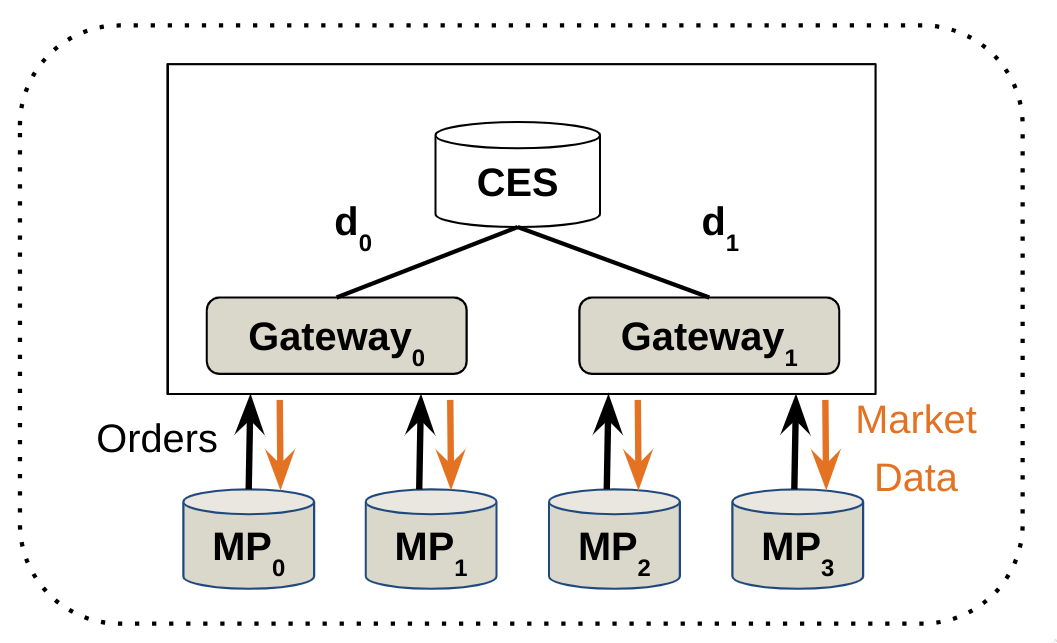
\includegraphics[width=0.4\textwidth]{./assets/architecture.png}
%     \caption{An Exchange's Infrastructure}
%     \label{fig:exchange}
%   \end{center}
% \end{figure}

\textbf{\textit{Gateways}}. The gateways are structures placed between traders
    and the CES. Their responsabilities consist of routing orders and market data, as 
    well as protecting the CES from abuse, e.g., unauthenticated or invalid orders. Within
    the on-premise clusters, gateways are made to be equidistant to the CES as to 
    ensure fairness regarding communication delays between themselves and the central exchange.

\begin{figure}[h!]
  \begin{center}
    \begin{minipage}{0.45\textwidth}
      \centering
      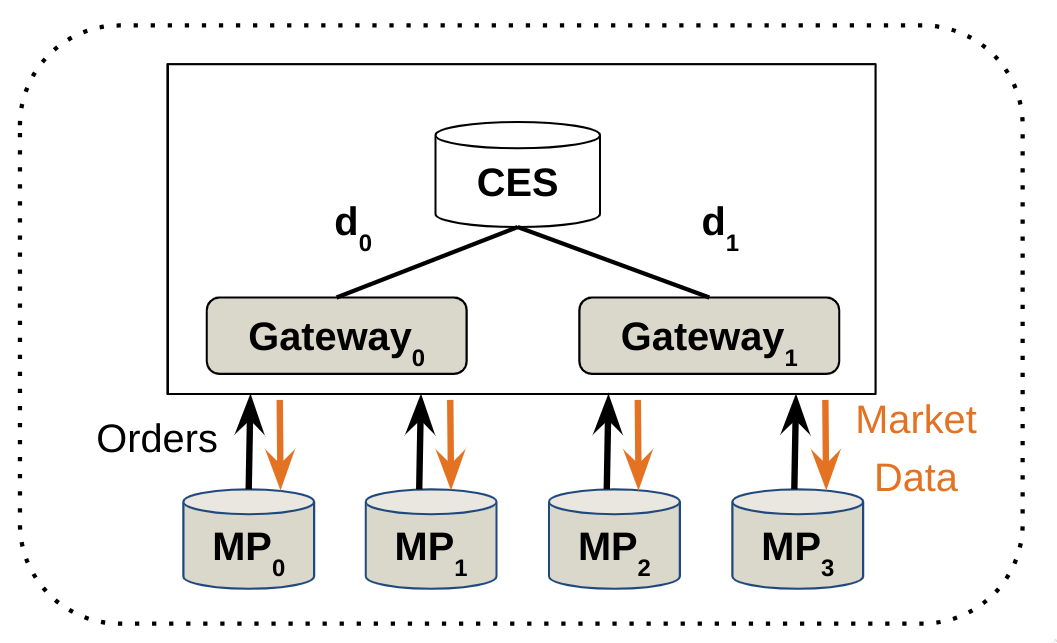
\includegraphics[height=0.20\textheight]{./assets/architecture.png}
      \caption{On-premise Datacenter}
      \label{fig:exchange}
    \end{minipage}
    \hfill
    \begin{minipage}{0.45\textwidth}
      \centering
      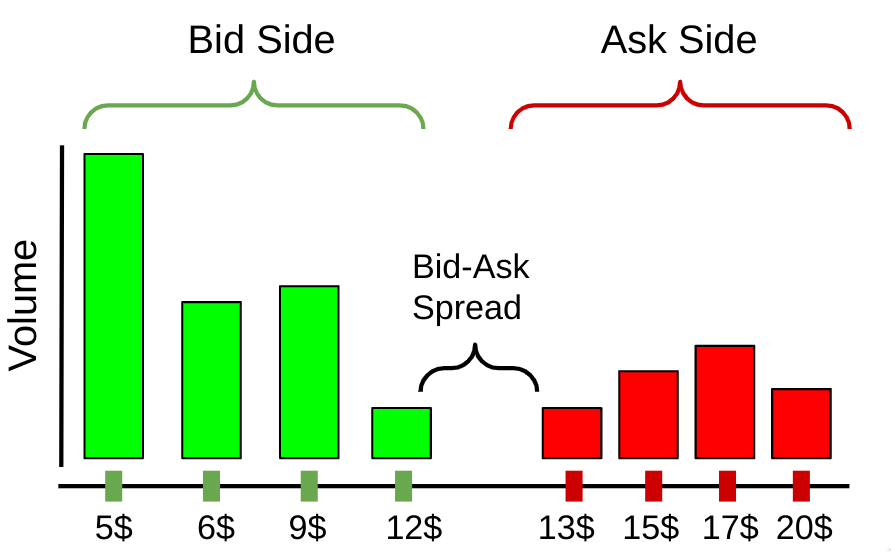
\includegraphics[height=0.20\textheight]{./assets/LOB.png}
      \caption{Limit Order Book}
      \label{fig:lob}
    \end{minipage}
  \end{center}
\end{figure}

\subsection{Migration to the Cloud}
Given the demanding network performance of financial exchanges, the use of 
on-premise data centers is the prevailing standard.
However, the cloud displays well-known advantages as a medium for communication. 
These include flexibility, scalability, robustness and potential cost savings. 
On the other hand, the public cloud also exhibits high latency variance \cite{cloudy}.
Additionally, it does not provide low-level engineering control to cloud-tenants such as switch-based multicast. 
As a result, cloud-based systems implement multicasting by directly unicasting a copy of a message 
to each recipient \cite{nezha, cloudex, octopus, dbo}.


A fundamental characteristic of a financial exchange is the ability to disseminate data
    to market participants in a fair manner. 
That is, all MPs receive updates to the market almost simultaneously, as to not allow 
    unwanted arbitrage opportunities.
Without native solutions to enable multicasting and the significant serial 
    delay of direct unicasting, a clear problem is presented 
    to achieve the possible migration of financial exchanges to the public cloud.

\subsection{Jasper: A Scalable Financial Exchange in the Cloud}
A siginificant project in this domain is Jasper \cite{jasper}, which offers 
a modern implementation of a financial exchange on the public cloud. 
This work realizes a multicast service that achieves low latency of less than 
250 µs and a latency difference of less than 1 µs across 1,000 multicast receivers.
To accomplish this, a series of techniques are employed.


\textbf{\textit{Overlay Proxy Tree}}. This is the starting point for Jasper's design 
    and borrow's the concept of trees to scale communication to a larger number of 
    receivers, while improving latency in comparison to direct unicasting \cite{matsuoka, twotree}.
    The structure of the tree with Depth (\textbf{D}) and fan-out (\textbf{F}) has been empirically established 
    as seen in Equations [\ref{eq:fanout}, \ref{eq:depth}].
    % Ideally, F has been fixed to 10, while the value of D is derived via [$log_{10}{(N)}$], where N is the number 
    % of receivers.

\begin{align}
F &= 10 \label{eq:fanout} \\
D &= \log_{10}{(N)} \label{eq:depth}
\end{align}

\textbf{\textit{Clock Synchronization}}. Jasper utilizes high-precision software clock 
 synchronization to compensate for noisy conditions in the cloud \cite{hyugens}. Additionally, 
 a common clock across a cluster allows for precise global timestamps to coordinate actions 
 across nodes.

\textbf{\textit{Hold and Release}}. Even with a proxy tree there still are serial delays that impact 
every hop in the system. Therefore, receivers located at the leaves of this tree will not receive 
packets simultaneously. By leveraging global timestamps, a technique called hold and release is 
applied where a chosen deadline is appended to every packet, instructing receivers when they are 
allowed to consume the data. That way, a temporal barrier is used to enforce simultanous updates from the 
market to all recipients. The deadline is set to a future point in time at which all receivers are highly likely 
to have received the message. To calculate these deadlines, the sender or root of the tree continuosly gathers
one-way-delay measurements between itself to all receivers in the tree.

\section{Cloud Computing}
Before personal computers became widespread, they were famously expensive 
for the everyday consumer. It wasn’t until the 1980s and 1990s 
that this changed. However, building large-scale applications 
still required significant knowledge in configuring, 
managing, and maintaining extensive computing resources.
In 2006, Amazon introduced Elastic Compute Cloud (EC2), 
a service that takes upon the responsability of providing and maintaining computational resources, 
which could be then rented to users per unit-time \cite{amazonEC2}.
EC2 offers units of compute, memory, and storage, 
all connected through a networking infrastructure allowing communication between these units. 
Through advancements in hardware virtualization, these resources could be allocated to 
developers through Virtual Machines (\textbf{VMs}) rather than being tied to specific physical instances.
This brought forth a paradigm well known today as cloud computing,
allowing for a more flexible use of compute, as machines could be up- and down-scaled 
more efficiently.
Many large corporations such as Google, IBM and Microsoft have followed and 
today the public cloud is an established medium for application deployment \cite{googleGCP, ibmCloud, Azure}.
Moreover, it is a significant technological industry, generating global 
spending that exceeds \$700 billion dollars per year \cite{cloudForecast}.

Despite the cloud's inherent flexibility, allowing applications to dynamically scale, 
works have shown that VMs with the same configuration often exhibit 
significant performance differences \cite{vmwareNUMA, longtails}. 
This variability is largely attributed to the cloud’s multi-tenant nature, 
where VMs may share CPU, memory, and network resources with other VMs. 
This resource contention can result in uneven performance, 
especially when one or more VMs, commonly referred to as \textit{"noisy neighbors"}, consume 
an excessive amount of shared resources.
These underperforming VMs, labeled as \textit{"stragglers"} in the literature, 
pose a challenge in maintaining predictable and efficient cloud-based computations. 
Stragglers can significantly delay the overall completion of tasks, particularly in 
environments where large-scale distributed computing takes place, reducing system throughput, 
causing inefficiencies, and ultimately leading to higher operational costs.

Research efforts have focused on mitigating the negative impact of 
straggler VMs in a cluster \cite{wrangler, selectingVMS, fasterJI}. 
These optimizations have been especially critical in the context of batch data 
processing frameworks, where task completion time can heavily depend on the 
performance of the slowest VM in the cluster.
As cloud infrastructure continues to evolve, ongoing research aims to 
further enhance the detection and handling of stragglers, ensuring that applications 
deployed in the cloud remain resilient and performant, even when encountering unpredictable resource contention.


% Early work sought to identify and manage stragglers within a cluster by 
% dynamically reallocating resources or rerouting tasks to more reliable VMs [YAK14]. 
% Other approaches aimed to predict the occurrence of stragglers and preemptively schedule tasks 
% across multiple VMs to minimize delays [YHG+17, YHGK15]. 


\subsection{LemonDrop}
One notable advancement in the field of optimizing straggler VMs is LemonDrop, 
designed to select and schedule virtual machines (VMs) based on an application's latency needs \cite{lemondrop}. 
LemonDrop utilizes an accurate clock synchronization algorithm,  
allowing it to detect fine-grained anomalies in one-way delays (OWD) between pairs of VMs \cite{hyugens}. 
This approach allows LemonDrop to uncover subtle performance variations that could otherwise go unnoticed. 

What distinguishes LemonDrop is its ability to frame the selection and scheduling process as a 
natural Quadratic Assignment Problem (QAP) \cite{QAP}. 
This allows an efficient assignment and scheduleing of the top-performing K VMs from a pool of N $>$ K
, optimizing both latency and overall performance. Unlike prior works that primarily focused on 
mitigating stragglers in batch processing, LemonDrop is particularly tailored to latency-sensitive applications, 
making it highly effective in real-time, interactive cloud environments. 
Furthermore, the system's ability to detect underperforming VMs
makes it valuable for autoscaling and maintaining application responsiveness.

% A relevant work in the domain of straggler optimization is LemonDrop, which is a method of selecting and scheduling
% VMs that is optimized for an applications latency needs \cite{lemondrop}.
% At the heart of LemonDrop lies a precise clock synchronization algorithm that detects subtle 
% anomalies in one-way delays (OWD) between virtual machine (VM) pairs. 
% Leveraging the communication patterns of the application, LemonDrop utilizes these inter-VM 
% OWD measurements to frame and address a natural Quadratic Assignment Problem \cite{QAP}, 
% enabling the selection and scheduling of the optimal K VMs from a pool of N $>$ K VMs.


\begin{algorithm}
\caption{FAQ Algorithm}\label{alg:faq}
\begin{algorithmic}[1]
\scalebox{0.7}{
\begin{minipage}{1.3\linewidth}
\Function{FAQ}{$\Lambda$, $\Delta$, $\epsilon$, $n$}
    \State $P^{(0)} = 1 1^T$
    \State $i = 0$
    \State $s = 0$
    \While{$s = 0$}
        \State $\nabla f(P^{(i)}) = -\Lambda P^{(i)} \Delta^T - \Lambda^T P^{(i)} \Delta$ \Comment{Gradient wrt current solution}
        \State $Q^{(i)} = \arg\min_{P \in \mathcal{D}} \text{trace}(\nabla f(P^{(i)})^T P)$ \Comment{Direction which minimizes 1st order approx of $f(P)$}
        \State $\alpha^i = \min_{\alpha \in [0,1]} f(P^{(i)} + \alpha Q^{(i)})$ \Comment{Best step size in chosen direction}
        \State $P^{(i+1)} = P^{(i)} + \alpha^i Q^{(i)}$ \Comment{Update our current solution}
        \State \textbf{if} $\|P^{(i)} - P^{(i-1)}\|_F < \epsilon$ \textbf{then} $s = 1$ \Comment{Stop opt}
        \State \textbf{if} $i > n$ \textbf{then} $s = 1$ \Comment{Stop opt}
        % \If{$\|P^{(i)} - P^{(i-1)}\|_F < \epsilon$}
        %     \State $s = 1$ \Comment{Stop opt}
        % \EndIf
        % \If{$i > n$}
        %     \State $s = 1$ \Comment{Stop opt}
        % \EndIf
        \State $i = i + 1$ \Comment{Iteration number}
    \EndWhile
    \State $P_{\text{final}} = \arg\min_{P \in \mathcal{P}} P^{(i-1)} P^T$
    \State \Return $P_{\text{final}}$
\EndFunction
\end{minipage}%
}
\end{algorithmic}
\end{algorithm}

\section{Motivation}
